\chapter{Introduction}
\label{chap:Introduction}
This chapter introduces the related literature review, motivation, and goals of the undertaken research.
The chapter begins with a brief preface of cryptology and its importance in the era Internet of Things (IoT) and Big Data.
In \secref{ch1_subsec_pkc} we present how Public-Key Cryptography (PKC) is shaping the security of our everyday life.
We introduce the importance of Pairing-Based Cryptography (PBC) in \secref{ch1_subsec_pbc} for the next generation of security protocols. 
\secref{ch1_sec_motivation} presents the motivation behind the works undertaken to assemble of this thesis.
\secref{ch1_sec_outline} outlines the overall organization of this thesis.

\section{Cryptology}
\label{chap:sec:crypto}
Cryptography is the science of communicating with the authentic receiver through an insecure channel in secret. 
Cryptanalysis is the techniques of breaking the secret communications.
Cryptology is the combination of these two domains.

The history of cryptography dates back to the time of the Greek and Roman empire.
Julius Caesar used a simple shift and substitute system.
Up until the early '70s of the last century, cryptology was evolved mostly for military purposes. 
The cryptography got its first democratic form in 1975 when Diffie and Hellman invented the concept of public-key cryptography \cite{diffie1976new}. 
The concept was first realized by as practical cryptosystem by the works of Rivest, Shamir and Adleman (RSA) in 1977 \cite{rivest1978method}.
At the same time in 1977, National Bureau of Standards published a cryptosystem intended for the governmental agencies or banks with the named Data Encryption Standard (DES).
From then a new era of cryptography known as \textit{Modern cryptography} was initiated.
The well-organized procedures called \textit{protocols} is the basis of Modern cryptography.
One of the most elegant features of modern crypto-protocols is their inner algorithms are not secret yet withstand cryptanalysis from experts/attackers.
More importantly, these protocols are easy to use for people with no understanding of the underlying principles.
For example, paying by credit cards or withdrawing money using debit cards with a personal identification number (PIN) is doable without concerning what’s going on under the hood. 

The little basic functionality of modern cryptosystem is to enable a sender (Alice \footnote{Alice and Bob are fictional characters first used by Rivest, Shamir and Adleman in \cite{rivest1978method} as placeholder name in cryptology.}) to convert a message (plaintext) into a cipher (ciphertext) before sending to a legitimate receiver (Bob) over the public communication media. 
The receiver can convert the cipher back into the original message using secret information named as a key.
An adversary (Eve) eavesdrops in the middle of the conversation to retrieve information from the cipher.
The cipher is safe from to the adversary until the key is not compromised. 

The security of modern cryptosystems depends not on the secrecy of the encryption algorithms but the difficulty of one-way problems. 
Such problems are easy to calculate in one direction but practically impossible to calculate in reverse direction in a reasonable amount of time using reasonable resources.
For example, let us consider a ciphertext $\cal{C}$ and a plaintext $\cal{P}$ and a 128-bit key $\cal{K}$. 
The encryption scheme $\cal{E}$ takes input $\cal{P}$ and $\cal{K}$ and output $\cal{C}=E( \cal{P}, K)$. 
To obtain the  key $\cal{K}$ from the $(\cal{P,C})$ pair, we need to try $2^{128} = 340,282,366,920,938,463,463,374,607,431,768,211,456 \approx 3.4 \times 10^{38}$ (39 decimal digits) combination of $128$-bit keys.
The most potent supercomputer till this date can compute 122.3 PETA ($10^{15}$) floating-point operations per second (PFLOPS).
Let us consider an optimistic assumption that 1000 (FLOPS) is required to check one key combination.
Under this assumption, the supercomputer can compute $122.3. \times 10^{15} / 1000 = 122.3 \times 10^{12}$ key combinations per second.
Then it will take about $3.4 \times 10^{38}/((122.3 \times 10^{12})(365 \times 24 \times 60 \times 60)) \approx  8.8 \times 10^{16}$ earth years.
According to the standard model of physical cosmology \cite{Ade:2015xua} the age of our universe is $13.8 \time 10^9$ or 13.8 billion years. 
It means finding a key using brute force search will require $6.3$ million years more than the age of the universe.
We can imagine how big the number $2^{128}$ is from this comparison.

Cryptography became more important as individuals and business increasingly depend on the Internet as a channel for communication. Therefore, the following four properties are the basis of a cryptosystem.


\begin{itemize}
\item Data confidentiality:
This property ensures that confidential information such as bank transactions or medical data etc. are secret from unauthorized entities. 

\item Data integrity:
When data is stored, this property ensures that it not only kept secret (Data confidentiality) but also not rigged.
Confidentiality and integrity is enforced by encryption.

\item Authentication:
In connection-oriented communication, authentication proves both parties identity before communication begins.
The digital signature is used for this purpose to sign a message electronically.
It shields the legitimate party against masquerader from impersonating as a trusted party.
This property gives the receiver a confidence to believe that the actual signee indeed sends the message sent over the insecure channel.

\item Non repudiation:
Non-repudiation (with proof of origin and with proof of receipt) ensures that the sender and receiver can not deny having taken part in communication.
Non-repudiation is essential for many cases especially e-commerce while communicating over the Internet.
\end{itemize}

The modern crypto-protocols fall into the following two major categories. 

\subsection{Symmetric/Private-Key Cryptography}
Private-Key Cryptography, also known Symmetric Cryptography is the technique where both the sender and the receiver use the same \textit{key} or easily derivable from one another to encrypt and decrypt a message.
This type of cryptography has an ancient history. 

Modern cryptosystems offer efficient symmetric cryptography algorithms, e.g Advanced Encryption Standard (AES) \cite{AES_DaemenR02}.
Such cryptography has two main obstacles i.e. \textit{Key management} and \textit{key establishment}.
Since the keys are same, they need to keep private (\textit{Key management})  in both ends and should be shared securely beforehand (\textit{Key establishment}) without physically meeting.

The Public-key Cryptography offers the solution for \textit{Key establishment} applying Diffie-Hellman key exchange.
This work primarily focuses on a specific type of Public-key Cryptography. 
The subsequent chapters will describe in details.

\subsection{Public-key Cryptography}
\label{ch1_subsec_pkc}
The inception of public-key cryptography solved the problem of key distribution of Symmetric-key cryptography.
It is also known as Asymmetric Cryptography.
The basic idea of public-key cryptography is to use two different keys for each communicating party.
One key is public-key which can be used by anyone to encrypt the message. 
The receiver needs the correlated private key to decrypt the message.
From a given public key and ciphertext it is asymptotically difficult to obtain the private key.

As aforementioned, In 1976, Whitfield Diffie and Martin Hellman published their monumental work as a key exchange  protocol\cite{diffie1976new}.  
\fgref{fig_DHKE} shows the simple overview of the Diffie-Hellman Key Exchange (DHKE).
The problems of key distribution and storage associated with symmetric cryptography were the motivation behind the concept of Asymmetric Cryptography, also referred to as Public- Key Cryptography. 

In brief, the protocol has two public parameters, the prime number $p$ and a generator $g$ known to all the parties involved in the communication.
The main idea is of this protocol is based on the difficulty to solve the one-way function, i.e., discrete logarithm.
Let's say, it is easy to calculate Alice public key $k_A$ using Alice private key $k_{Ad}$ as $k_A = g^{k_{Ad}} (\bmod ~p).$ 
However, it will be difficult to obtain $k_{Ad}$ from $k_A, g$ and $p$.
In other words, it is easy to calculate the public key from the private key, but the reverse process is practically impossible.
Using this key-exchange, we change to establish a shared secret which we can for further encrypted communication.

  \begin{figure}
	\centering
	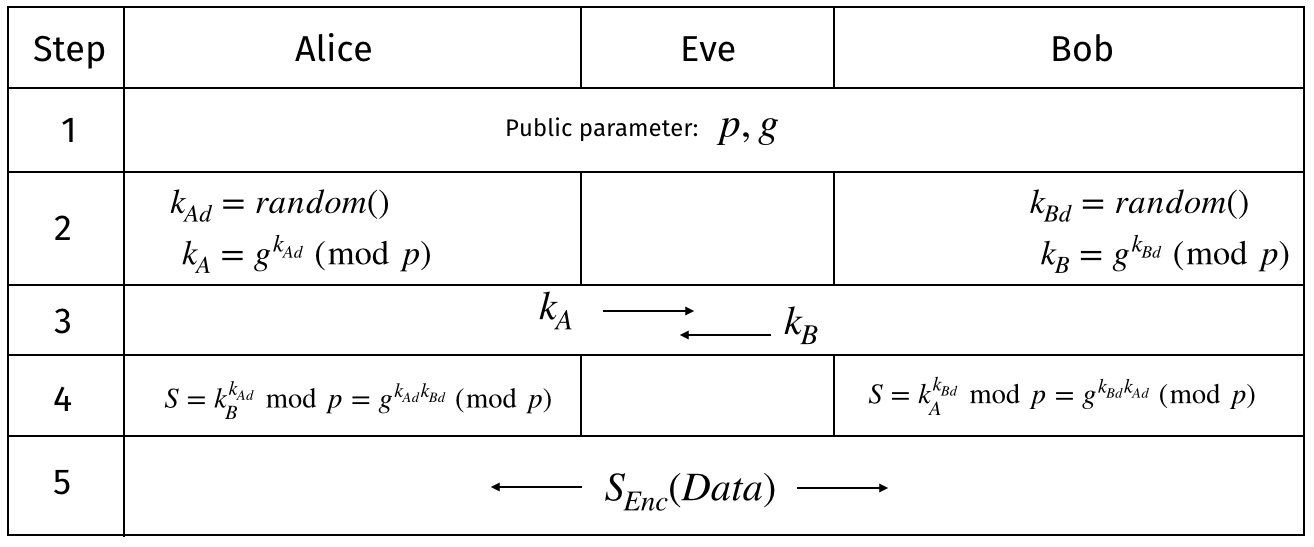
\includegraphics[width=.9\linewidth, height=.67\textheight, keepaspectratio]{Figures/DHKE}
	\caption{Exchanging shared secret key using DH-key exchange.}
	\label{fig_DHKE}
\end{figure}

Rivest, Shamir, and Adleman (RSA) realized this protocol in 1977 and published their magnum opus which is widely known as RSA cryptosystem \cite{rivest1978method}. 
The security of the RSA depends on the difficulty of factorization of a larger integer into its two prime factors and the trapdoor permutation for encryption.
Let us denote two large primes $p$ and $q$ (in practice about 1000-bit).
It is easy to calculate their product to get $n = pq$.
The reverse process that is for a given integer $n$ it will be arduous to retain $p$ and $q$.
Using the state-of-the-art integer factoring algorithm \textit{general number field sieve }(GNFS), it will take approximately $2^{90}$ basic operation to factor a 2048-bit integer.
After more than 40 years of the RSA breakthrough, it is still standing as an epitome of public key cryptography.
Besides encryption, RSA also enables \textit{digital signature }where the sender uses his private key to sign a message, and the receiver verifies the signature by the senders public key. 
Verification of a digitally signed message gives the receiver the confidence that a senders private key is tied to his public key.
It is done to prevent forgery and holds \textit{Non-repudiation} property.

In the mid 80's the independent work of Miller \cite{C:Miller85} and Koblitz \cite{koblitz1987elliptic} began the journey of elliptic curve cryptosystems (ECC). 
The security of elliptic curve cryptography protocols depends on the difficulty to solve elliptic curve discrete logarithm problem.
The mathematical details of this problem appear in Chapter 2. %TODO
ECC provides a shorter key length for the same level of security than RSA which makes ECC  popular among the researchers. 
Compared to RSA, ECC has other advantages. 
While RSA provides encryption and digital signature; ECC has a family of algorithms for encryption, signature, key agreement and some advanced high-level cryptographic protocols such as ID-based encryption \cite{AC:BonLynSha01}, where user's unique ID, e.g. email address, can be used as a public key. 
The high-level cryptographic functionalities are provided by paring over elliptic curves \cite{book_GPCMrabet2016} which brings a new paradigm in cryptography called pairing-based cryptography.

\subsection{Pairing-Based Cryptography}
\label{ch1_subsec_pbc}
Since the inception by Sakai et al. \cite{sakai2000cryptosystems}, pairing-based cryptography has gained much attention to cryptographic researchers as well as  to mathematicians. It gives flexibility to protocol researcher to innovate applications with provable security and at the same time to mathematicians and cryptography engineers to find efficient algorithms to make pairing implementation more efficient and practical.

Generally, a pairing is a bilinear map $e$ typically defined as  $\g1 \times \g2 \to \g3$, where $\g1$ and $\g2$ are additive cyclic sub-groups of  order $r$  on a certain elliptic curve $E$ over a finite extension field $\FPK$ and $\g3$ is a multiplicative cyclic group of order $r$ in $\mF{p}{k}$.
Let $E(\Fp)$ be the set of rational points over the prime field $\Fp$ which forms an additive Abelian group together with the point at infinity $\cal{O}$. The total number of rational points is denoted as $\#E(\Fp)$. Here, the order $r$ is a large prime number such that $r | \#E(\Fp)$ and gcd$(r,p)=1$. The embedding degree $k$ is the smallest positive integer such that $r | (p^k -1)$.
Two fundamental properties of pairing are
\begin{itemize}
	\item bilinearity is such that $\forall P_i \in \g1$ and $\forall Q_i \in \g2$, where $i= 1, 2$, then $e(Q_1+Q_2,P_1) = e(Q_1,P_1). e(Q_2,P_1)$ and $e(Q_1,P_1+P_2) = e(Q_1,P_1). e(Q_1,P_2)$,
	\item and $e$ is non-degenerate means $\forall P \in \g1$ there is a $Q \in \g2$ such that  $e(Q,P) \neq 1$ and $\forall Q \in \g2$ there is a $P \in \g1$ such that $e(P,Q) \neq 1$.
\end{itemize}
Such properties allows researchers to come up with various cryptographic applications including ID-based encryption \cite{C:BonFra01}, group signature authentication \cite{C:BonBoySha04}, and functional encryption \cite{C:OkaTak10}.  However, the security of pairing-based cryptosystems depends  on 
\begin{itemize}
	\item  the difficulty of solving elliptic curve discrete logarithm problem (ECDLP) in the groups of order $r$ over $\Fp$,
	\item  the infeasibility of solving the discrete logarithm problem (DLP) in the multiplicative group $\g3 \in \mF{p}{k}$,
	\item and the difficulty of pairing inversion.
\end{itemize}
To maintain the same security level in both groups, the size of the order $r$ and extension field $p^k$ is chosen accordingly. If the desired security level is $\delta$ then $\log_2 r  \geq 2\delta$ is desirable due to Pollard's rho algorithm \cite{1978-pollard-kangaroo}.  For efficient pairing, the ratio $\rho = \log_2 p^k/ \log_2 r \approx 1$,   is expected (usually  $1\leq  \rho  \leq 2$). In practice, elliptic curves with small embedding degrees $k$ and large $r$ are selected and commonly are knows as ``pairing-friendly" elliptic curves.

Galbraith et al. \cite{galbraith2008pairings} have classified pairings as three major categories based on the underlying group's structure as 
\begin{itemize}
	\item Type 1, where $\g1 = \g2$, also known as symmetric pairing. 
	\item Type 2, where $\g1 \neq \g2$, known as asymmetric pairing. There exists an efficiently computable isomorphism $\psi : \g2 \to \g1$ but none in reverse direction.
	\item Type 3, which is also asymmetric pairing, i.e., $\g1 \neq \g2$. But no efficiently computable isomorphism is known in either direction  between $\g1$ and $\g2$.
\end{itemize}


%This thesis chooses one of the Type 3 variants of pairing named as Optimal-Ate \cite{DBLP:journals/tit/Vercauteren10} with Kachisa-Schaefer-Scott (KSS) \cite{EPRINT:KacSchSco07} pairing-friendly curve of embedding degree $k=16$. 
%Few previous works have been done on this  curve. 
%Zhang et al. \cite{INDOCRYPT:ZhaLin12} have shown the computational estimation of the Miller's loop and proposed efficient final exponentiation for 192-bit security level in the context of Optimal-Ate pairing over KSS-16 curve. 
%A few years later Ghammam et al. \cite{EPRINT:GhaFou16b} have shown that KSS-16 is the best suited for multi-pairing (i.e., the product and/or the quotient) when the number of pairing is more than two. 
%Ghammam et al. \cite{EPRINT:GhaFou16b} also corrected the flaws of proposed final exponentiation algorithm by Zhang et al. \cite{INDOCRYPT:ZhaLin12} and proposed a new one and showed the vulnerability of Zhang's parameter settings against small subgroup attack. 
%The recent development of NFS by Kim and Barbulescu \cite{C:KimBar16} requires updating the parameter selection for all the existing pairings over the well known pairing-friendly curve families such as BN \cite{SAC:BarNae05}, BLS \cite{EPRINT:FreScoTes06} and KSS \cite{EPRINT:KacSchSco07}.
%The most recent study by Barbulescu et al. \cite{EPRINT:BarDuq17} have shown the security estimation of the current parameter settings used in well-studied curves and proposed new parameters, resistant to small subgroup attack.
%
%Barbulescu and Duquesne's study finds that the current parameter settings for 128-bit security level on BN-curve studied in literature can withstand for 100-bit security. 
%Moreover, they proposed that BLS-12 and surprisingly KSS-16 are the most efficient choice for Optimal-Ate pairing at the 128-bit security level. Therefore, the authors focus on the efficient implementation of the less studied KSS-16 curve for Optimal-Ate pairing by applying the most recent parameters.
%Mori et al. \cite{PAIRING:MANS13} and Khandaker et al. \cite{ICISC:KONSD16} have shown a specific type of sparse multiplication for BN and KSS-18 curve respectively where both of the curves supports sextic twist. 
%The authors have extended the previous works for quartic twisted KSS-16 curve and derived pseudo-8 sparse multiplication for line evaluation step in the Miller's algorithm. 
%As a consequence, the authors made the choice to concentrate on Miller's algorithm's execution time and computational complexity to verify the claim of \cite{EPRINT:BarDuq17}.
%The implementation shows that Miller's algorithm time has a tiny difference between KSS-16 and BLS-12 curves. However, they both are more efficient and faster than BN curve. 
\section{Motivation}
\label{ch1_sec_motivation}

This section outlines the overall motivation behind the undertaken works.
In this course, some mathematical notations will appear without detailed definitions.
The subsequent chapters will define them with further elaboration.
Let us consider the following two cases.

\subsection*{Case 1: IoT Security}
Human civilization is moving to a direction where data generated from the devices used in our daily life will define how smart our society will be.
In technical jargon, we define that IoT (Internet of Things) era controlled by Data Science.
Some data can be mundane with no purpose, and some data can be extraordinarily important.
Let us imagine a case where the adversary takes controls heartbeat monitor sensor of our smartwatch or control sensors of a self-driving car.
The outcome of the damage is unimaginable. 
There is no alternative to protect these data from unwanted access.
The challenge is, most of the IoT devices are equipped with small sensors.
Such devices are computationally resource constrained.
In some devices, it is somewhat impractical to generate key pairs for widely practiced security protocols.
There are several innovative solutions such as Identity-based encryption that can use device's unique ID as a key.
The applications mentioned above stand on a compelling branch of cryptography named \textit{pairing-based cryptography over elliptic curve}.


\subsection*{Case 1: Security of Medical Data in Cloud}
Modern medical diagnosis depends on medical examination that produces a vast amount of data ranges from patients personal information to diagnosis reports and images.
Most of the data are stored in large cloud-based databases. 
For the privacy of the patient, they should be encrypted before stored.
By analyzing such medical data, it is possible to predict the probability of a patient's vulnerability to a particular disease. 
However, it is not always the doctor who examined the patient can do that.
Sometimes third-party researchers are interested in such data-set. 
However, the identity of the patient should not be obtained by any third-party using that data. 
One solution for this case is any third party can search data and perform the mathematical operation in the encrypted database without decrypting the data.
This scenario can be realized by using homomorphic encryption which is also powered by pairing-based cryptography.

However, pairing-based cryptography is a complex mathematical process.
To practically apply it, we need to carry out its fundamental algorithms more efficiently.
In this thesis, our objective is to improve and find out more efficient algorithms that can realize high-level of security protocols.

\section{Our Contribution}
\label{ch1_sec_contribution}
As discusses above, pairing is a bilinear map from two groups $\mathbb{G}_1$ and $\mathbb{G}_2$ to a group $\mathbb{G}_3$, where they have respectively same prime order $r$.
In detail, $\mathbb{G}_1$ and $\mathbb{G}_2$ respectively becomes a subgroup in an elliptic curve group $E(\F{q}{})$ and $E(\F{q}{k})$, and $\mathbb{G}_3$ becomes a subgroup in $\F{q}{k}$, where $q$ is a power of $p$ and an extension degree $k$ is especially called the {\it embedding degree}.

In pairing-based cryptography, there exists several predominant operations which are the bottleneck for any pairing-based protocols.
These operations are Miller's algorithm, final exponentiation in $\mathbb{G}_3$, scalar multiplications in $\mathbb{G}_1$ and $\mathbb{G}_2$, and exponentiation in $\mathbb{G}_3$.
The calculation costs of pairing and scalar multiplication in $\g{2}$ are the significant costs among the operations required for pairing-based cryptographies.
Therefore, efficient Miller's algorithm and scalar multiplications in $\mathbb{G}_2$ can reduce the total cost of pairing-based cryptography.
In this work, we focus on these operations especially Miller's algorithm and scalar multiplications in $\mathbb{G}_2$.
	
In this thesis, we focus on Type 3 pairing that is asymmetric pairing such as Ate \cite{EPRINT:MKHO07} and Optimal-Ate \cite{DBLP:journals/tit/Vercauteren10} pairing.
Therefore, we have not efficient homomorphic map from $\g{1}$ to $\g{2}$. 
Generally, in asymmetric pairing the scalar multiplication is carried out over efficiently calculable group $\g{1}$ and then the result is mapped to $\g{2}$.

The {\it embedding degree} is an important parameter that determines the security level of pairing-based cryptographies.
Therefore, to achieve efficient pairing on ordinary curves whose {\it embedding degree} are flexibly selectable are required.
This thesis targets Ate and {\it twisted} Ate pairings because they are efficiently calculated on normal pairing-friendly curve Kachisa-Schaefer-Scott (KSS) \cite{EPRINT:KacSchSco07}.
Ate and Optimal-Ate are use calculated over certain elliptic curve groups $\g{1}$ and $\g{2}$.
In this thesis, we accelerate scalar multiplications in $\g{2}$ group which can be extended in $\g{1}$

In the case of scalar multiplication, we reduce the number of elliptic curve doubling by decomposing a scalar with a key relation for KSS curves.
Besides, we proposed state-of-the-art Miller's algorithm calculation at the 128-bit security level.

Our proposed methods can substantially improve pairing calculation.
Therefore, our research contributes to committing high-level security for sophisticated protocols, e.g. ID-based or Homomorphic encryption.

\section{Thesis Outline}
\label{ch1_sec_outline}
This thesis is organized as follows: 

In Chapter 2, we briefly discuss the mathematical concepts that are related to understanding the concepts of this thesis.
We also define the pairing in general. 
Besides, a target class of pairing-friendly elliptic curves is shown.

Chapter 3 proposes an efficient Optimal-Ate pairing for KSS-18 curve. 
We improved the Miller's algorithm of Optimal-Ate pairing by proposing \textit{pseudo 12-sparse multiplication} multiplication.
In order to evaluate our theoretic proposal, we also include some experimental results with recommended parameter settings.

Chapter 4 proposes a technique that will accelerate scalar multiplications in $\g{2}$ over KSS-18 curve. 
It is crucial to derive efficiently computable endomorphisms for accelerating scalar multiplication.
The target $\g{2}$ group has a property that specific scalar multiplication can utilize  Frobenius endomorphism that is efficiently computable.
Focusing on this property, we derive an essential relation available for scalar multiplication in $\g{2}$ from the structural properties of target elliptic curve.
Then, using the relation, efficient scalar multiplication is proposed together with multi-scalar multiplication.
Besides, from the experimental results, we show that the proposed scalar multiplication is about 60 times faster than the conventional method.  

In chapter 5, we derived twist property for target elliptic curves for 192-bit security level and compared their performances concerning scalar multiplication.
This thesis shows that sextic twist over KSS-18 curve has an advantage over quartic twist in KSS-16 curve.

Chapter 6, shows the state-of-the-art improvement of Optimal-Ate pairing over KSS-16 curve at the 128-bit security level.
We adopted the most recent parameter and theoretically derived most efficient pairing calculation.
Besides, we also showed experimental implementation and compared our result with other pairing-friendly curves.


In Chapter 7, we opt to further accelerate the work of chapter 6 by improving the finite field arithmetic using cyclic vector multiplication algorithm.
We showed comparative results between chapter 6's proposal and this. 
We also showed memory optimization currently exists final exponentiation algorithm.

Chapter 8 shows the   $\g{2}$  scalar multiplication with by applying different dimension of GLV decomposition.
We showed theoretical and experimental result and showed that 4-dimension is optimal for efficient scalar multiplication in  $\g{2}$ in KSS-16 curve.

Finally, Chapter 9 concludes this thesis.

	
